
Das Mobile Game "PONG" wird im Wintersemester 2022/2023 im Rahmen der Lehrveranstaltung
"Software Engineering“ in dem Studiengang „Informatik” des Fachbereiches 5 (Elektrotechnik und
Informationstechnik) an der Fachhochschule Aachen entwickelt.
Der Fachbereich befindet sich in der Eupener Straße 70 in D-52066 Aachen.

Die finale Version dieses Dokumentes muss bis zum \textbf{11.11.2022} fertiggestellt und
von beiden Seiten unterzeichnet werden.

Bis zum \textbf{21.12.2022} muss eine \gls{beta} erstellt werden, die dem Kunden
vorgelegt werden kann. 
Die erste \gls{release} der Applikation muss bis Ende
des Wintersemesters 2022/23, zum \textbf{12.01.2023}, fertiggestellt und abgenommen werden.

Zur Fertigstellung des Projekts haben wir als Auftragnehmer ein Zeitbudget von 600 Stunden. 


\begin{figure}[h!]
    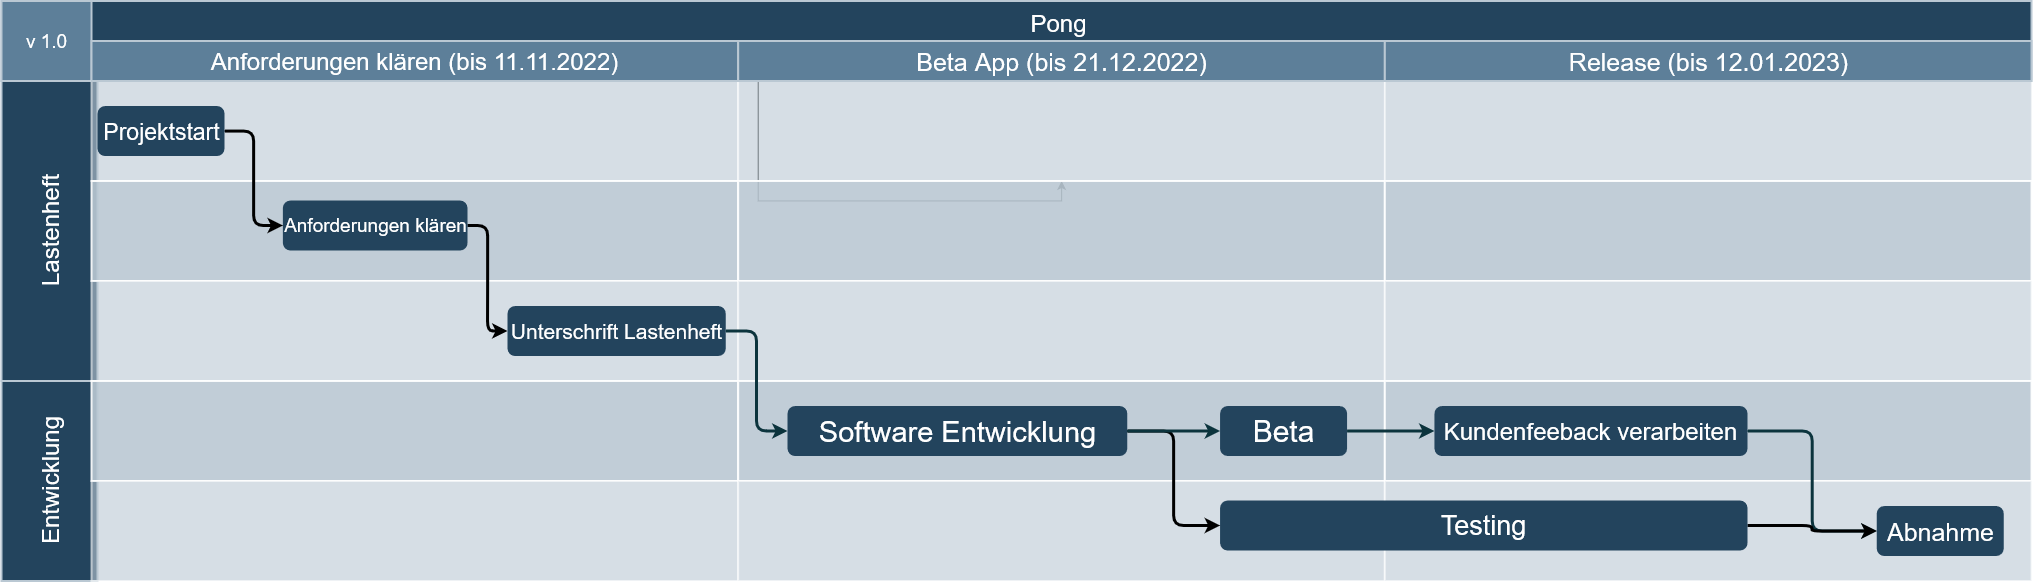
\includegraphics[width=\textwidth]{pics/ZeitlicherAblauf.png}
\end{figure}

